%%%%%latex preamble%%%%%
\documentclass[titlepage]{article}\usepackage[]{graphicx}\usepackage[]{color}
%% maxwidth is the original width if it is less than linewidth
%% otherwise use linewidth (to make sure the graphics do not exceed the margin)
\makeatletter
\def\maxwidth{ %
  \ifdim\Gin@nat@width>\linewidth
  \linewidth
  \else
  \Gin@nat@width
  \fi
}
\makeatother


\usepackage{listings}
\definecolor{mygreen}{rgb}{0,0.6,0}
\definecolor{mygray}{rgb}{0.5,0.5,0.5}
\definecolor{mymauve}{rgb}{0.58,0,0.82}
\lstset{ %
  backgroundcolor=\color{white},   % choose the background color; you must add \usepackage{color} or \usepackage{xcolor}
  basicstyle=\footnotesize,        % the size of the fonts that are used for the code
  breakatwhitespace=false,         % sets if automatic breaks should only happen at whitespace
  breaklines=true,                 % sets automatic line breaking
  captionpos=b,                    % sets the caption-position to bottom
  commentstyle=\color{mygreen},    % comment style
  deletekeywords={...},            % if you want to delete keywords from the given language
  escapeinside={\%*}{*)},          % if you want to add LaTeX within your code
  extendedchars=true,              % lets you use non-ASCII characters; for 8-bits encodings only, does not work with UTF-8
  frame=single,                    % adds a frame around the code
  keepspaces=true,                 % keeps spaces in text, useful for keeping indentation of code (possibly needs columns=flexible)
  keywordstyle=\color{blue},       % keyword style
  language=Python,                 % the language of the code
  morekeywords={*,...},            % if you want to add more keywords to the set
  numbers=left,                    % where to put the line-numbers; possible values are (none, left, right)
  numbersep=5pt,                   % how far the line-numbers are from the code
  numberstyle=\tiny\color{mygray}, % the style that is used for the line-numbers
  rulecolor=\color{black},         % if not set, the frame-color may be changed on line-breaks within not-black text (e.g. comments (green here))
  showspaces=false,                % show spaces everywhere adding particular underscores; it overrides 'showstringspaces'
  showstringspaces=false,          % underline spaces within strings only
  showtabs=false,                  % show tabs within strings adding particular underscores
  stepnumber=2,                    % the step between two line-numbers. If it's 1, each line will be numbered
  stringstyle=\color{mymauve},     % string literal style
  tabsize=2,                       % sets default tabsize to 2 spaces
  title=\lstname                   % show the filename of files included with \lstinputlisting; also try caption instead of title
}
\usepackage{alltt}
\usepackage[sc]{mathpazo}
\usepackage{amsmath, amsthm, amssymb}
\usepackage{graphicx}
\usepackage[T1]{fontenc}
\usepackage{geometry}
\geometry{verbose,tmargin=2.5cm,bmargin=2.5cm,lmargin=1.5cm,rmargin=1.5cm}
\setcounter{secnumdepth}{2}
\setcounter{tocdepth}{2}
\usepackage{url}
\usepackage[unicode=true,pdfusetitle,
  bookmarks=true,bookmarksnumbered=true,bookmarksopen=true,bookmarksopenlevel=2,
breaklinks=false,pdfborder={0 0 1},backref=false,colorlinks=false]
{hyperref}
\hypersetup{pdfstartview={XYZ null null 1}}
\usepackage{float}
\usepackage{bm}
\usepackage{tikz}
 %changes default sectioning commands -> 1,a, etc.
%\usepackage{breakurl}
\renewcommand{\thesubsection}{(\alph{subsection})}
\renewcommand{\thesubsubsection}{\roman{subsection}.}
\usepackage{lastpage}
\usepackage{fancyhdr}
\pagestyle{fancy}
\usepackage{tikz-qtree}

%%% Header and Footer %%% 
\lhead{}
\chead{\leftmark}
\rhead{}
\lfoot{Aaron Gonzales; Algorithms}
\cfoot{Homework X}
\rfoot{Page \thepage\ of \pageref{LastPage}}
\IfFileExists{upquote.sty}{\usepackage{upquote}}{}

\begin{document}

\title{Homework 7, CS561, Fall 2014}
\author{Aaron Gonzales}
%\maketitle


%%%% useful align for this
\section{26.2 - 4: Min cut/Max flow}
  \begin{quote}
    \textbf{In the example of Figure 26.6, what is the minimum cut corresponding
    to the maximum flow shown? Of the augmenting paths appearing in the
    example, which one cancels flow?}
  \end{quote}

  \begin{figure}
    \begin{center}
    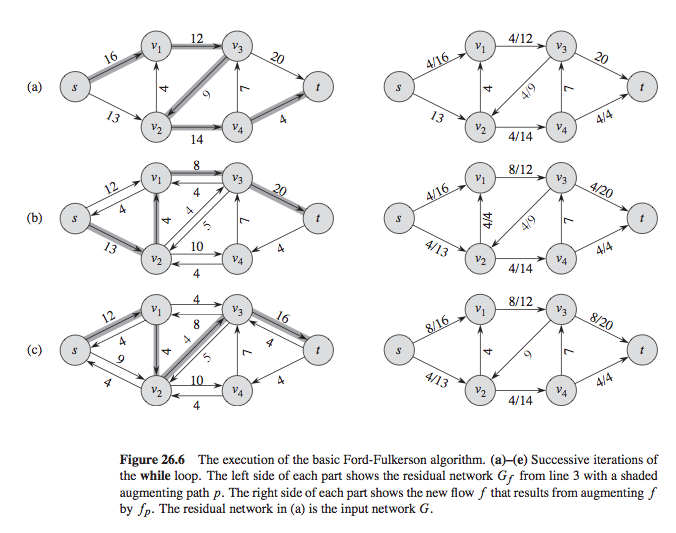
\includegraphics[scale=0.40]{26.6a.png}\\*
    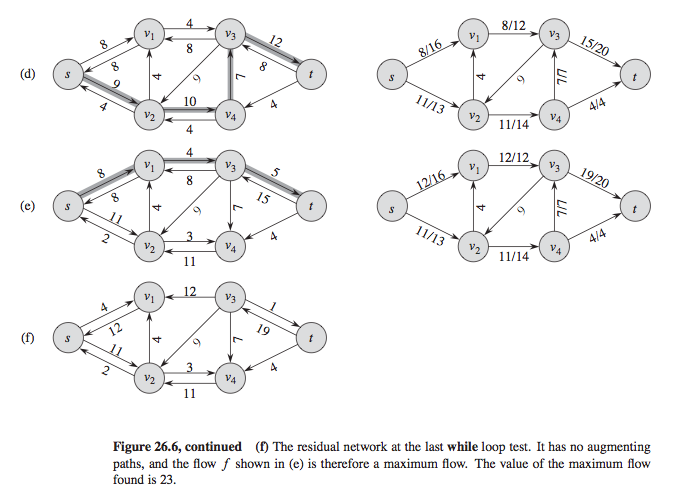
\includegraphics[scale=0.40]{26.6b.png}\\*
  \end{center}
  \end{figure}
  \subsubsection{Answer:}
  \vspace{9cm}


\section{26.2 - 11 : connectivity}
  \begin{quote}
    \textbf{The edge connectivity of an undirected graph is the minimum number
      $k$ of edges that must be removed to disconnect the graph. For example,
      the edge connectivity of a tree is 1, and the edge connectivity of a
      cyclic chain of vertices is 2. Show how to determine the edge
      connectivity of an undirected graph $G = (V,E) $ by running a
      maximum-flow algorithm on at most $|V|$ flow networks, each having $O(V)$
      vertices and $O(E)$ edges.}
  \end{quote}

  \subsubsection{Answer:}
  \vspace{9cm}


\section{Perfect Matchings}
  \begin{quote}
      \textbf{A bipartite graph is a graph that contains no cycle with an odd
      number of edges. Recall from the wrestler problem that a graph, $G = (V,
      E)$ is
    bipartite iff $V$ can be partitioned into two sets $L, R$ such that all
    edges in $E$
    have one endpoint in $L$ and one endpoint in $R$. A matching in a graph is a set of
    edges $E' \in E$ such that each vertex in $V$ is matched at most once, i.e. it is
    incident to a most one edge in $E'$. A perfect matching is a matching where every
    vertex is matched, i.e. is incident to exactly one edge in $E'$. For a set of
    vertices $S \in V$, let $N(S)$ be the set of all neighbors of $S$, i.e. $\{y
    \in V : (x,y) \in \, E $ for some $x \in S\}$ \\*
    Assume we are given a bipartite graph where $|L| = |R|$. Prove that there is a
    perfect matching in $G$ iff $|N(S)| \geq |S|$ for all $S \in L$.
    Hint: Use the Max flow/Min Cut Theorem}
  \end{quote}
  \subsubsection{Answer:}
  \vspace{9cm}



\section{Image segmentation}
  \begin{quote}
    \textbf{Consider the following problem related to segmenting the pixels
      of an image between foreground and background. We have a picture that
      consists of $n$ pixels. We represent this as an undirected graph $G =
      (V,E)$ where $V$ is the set of pixels and there is an edge $(i,j) \in
      E$ iff pixel $i$ and pixel $j$ are neighbors in the image
      \footnote{Note that we'd commonly expect this graph to be a grid, but
        in fact we want to handle any arbitrary graph (to handle, e.g., 3-D
        images, wrapped and warped images, etc)}}. \\* 
        \textbf{We want to find
        a good segmentation, which is an assignment of each pixel to either
        the foreground or the background.  For each pixel $i$, we have a
        likelihood $a_i$ that $i$ belongs to the foreground and a likelihood
        $b_i$ that $i$ belongs to the background. These likelihood values are
        all non-negative. Additionally, for each edge $(i, j) \in E$, we have
        a non-negative separation penalty $p_i,j$ which is charged if one of
        $i$ or $j$ is assigned to the foreground and the other is assigned to
        the background.  Our problem then is to find a partition of the set
        of pixels into sets $A$ and $B$ so as to maximize:}
    \[ L(A, B) = \sum_{i \in A}  a_i + \sum_{i \in B} b_i − \sum_{(i,j) \in E, | A \cap \{i,j\} | = 1} p_{i,j} \]
      \textbf{Give an efficient algorithm to solve this problem}
  \end{quote}

  \subsubsection{Answer:}

  \vspace{9cm}


\section{Exercise 29.2-2 (Linear Program)}
  \begin{quote}
    \textbf{Write out explicitly the linear program corresponding to finding
    the shortest path from node $s$ to node $y$ in Figure 24.2(a).}
  \end{quote}
\usetikzlibrary{arrows}
\begin{figure}
  \begin{center}
	\begin{tikzpicture}[->,>=stealth',shorten >=1pt,auto,node distance=3cm,
	  thick,main node/.style={circle,fill=blue!20,draw,font=\sffamily\Large\bfseries}]

	  \node[main node] (1) {3};
	  \node[main node] (2) [right of=1] {9};
	  \node[main node] (3) [below of=2] {11};
	  \node[main node] (4) [below of=1] {5};
	  \node[main node] (5) [below left of=1] {0};

	  \path[every node/.style={font=\sffamily\small}]
		(1) edge node [above] {6} (2)
			 edge [bend right] node[left] {2} (4)
			%edge [loop above] node {0.1} (1)
		(2) edge[bend right] node [bend right] {2} (3)
			%edge [loop left] node {0.4} (2)
			%edge [bend right] node[left] {0.1} (3)
		(3) edge [bend right] node [right] {7} (2)
                    edge node [below right] {3} (5)
		(4) edge [bend right] node [above left] {1} (1)
                        edge node[below] {6} (3)
                        edge node {4} (2)
		(5) edge node [above left] {3} (1)
                    edge node [below left] {5} (4);
                    %edge node [left] {5} (2);
			%edge [loop right] node {0.6} (4)
	\end{tikzpicture}
  \end{center}
\caption{Figure 24.2 from CLRS}
\label{fig:figure1}
\end{figure}

  \subsubsection{Answer:}
  \vspace{9cm}

\section{Exercise 29.2-4 (Network Flow as an LP)}
  \begin{quote}
    \textbf{Write out explicitly the linear program corresponding to finding
    the maximum flow in Figure 26.1(a).}
  \end{quote}
  \begin{figure}
    \begin{center}
    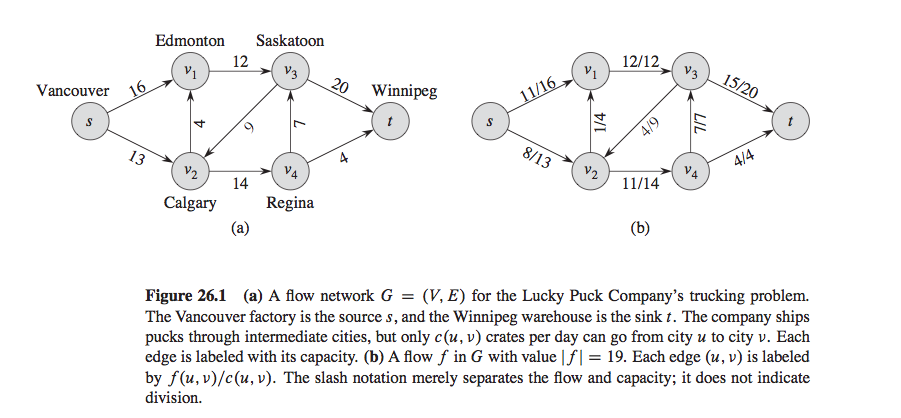
\includegraphics[scale=0.40]{26.1a.png}\\*
    \end{center}
  \end{figure}

  \subsubsection{Answer:}
  \vspace{9cm}
\section{Rock, Paper, Scissors}
  \begin{quote}
    \textbf{Rock, Paper, Scissors is a simple 2 person game. In a given round,
    both players simultaneously choose either Rock, Paper or Scissors. If they
    both choose the same object, it’s a tie. Otherwise, Rock beats Scissors;
    Scissors beats Paper; and Paper beats Rock. Imagine you’re playing the
    following betting variant of this game with a friend. When Scissors beats
    Paper, or Paper beats Rock, the loser gives the winner \$1. However, in the case
    when Rock beats Scissors, this is called a \textbf{smash}, and the loser must give the
    winner \$10.}
  \end{quote}

  \begin{itemize}
    \item \textbf{Say you know that your friend will choose Rock, Scissors or
        Paper, each with probability $\frac{1}{3}$. Write a linear program to
        calculate the probabilities you should use of choosing each object in
        order to maximize your expected winnings. Let $p_1,p_2,p_3$ be variables
        associated with the best way of choosing Rock, Scissors and Paper
        respectively. Note: If you want to check your work, there are several free
        linear program solvers on the Internets: check the Wikipedia page on linear
        programming.} 
      \item \textbf{Now say that your friend is smart and, also,
        clairvoyant: she will magically know the exact probabilities you are
        using and will respond optimally. Write another linear program to
        calculate the probabilities you should now use in order to maximize your
        expected winnings. \\* Hint 1: If your opponent knows your strategy, her
        strategy will be to choose one of the three objects with probability 1.
      \\* Hint 2: Review the LP you wrote for the shortest paths problem.}
  \end{itemize}
  \subsubsection{Answer:}

  \vspace{9cm}

\section{Independent-Set}
  \begin{quote}
  \textbf{The problem INDEPENDENT-SET asks: Does there exist a set of $k$
  vertices in a graph $G$ with no edges between them? Show that this problem is
  NP-Complete. (hint: Reduce from CLIQUE)}
  \end{quote}
  \subsubsection{Answer:}

  \vspace{9cm}








\section{Exercise 34.5-1 (Subgraph Isomorphism)}
  \begin{quote}
    \textbf{The subgraph-isomorphism problem takes two undirected graphs $G_1$ and
    $G_2$, and it asks whether $G_1$ is isomorphic to a subgraph of $G_2$. Show that the
    subgraph-isomorphism problem is NP-complete.}
  \end{quote}

  \subsubsection{Answer:}
  \vspace{9cm}
\end{document}


\end{document}
